\section{Sistema de archivos}
\label{sec::filesystem}

Para permitir cargar tareas desde disco duro, se hace necesario contar con una manera de
abstraer una jerarqu\'ia de archivos por sobre la organizaci\'on de bits en sectores que
corresponde al nivel de abstracci\'on de un controlador de disco duro. Para ello se
implement\'o un sistema de archivos.

Nos debatimos entre dos sistemas de archivos: El sistema de archivos VFAT 16, que consiste
en FAT 16 pero con \textit{hack} que permite nombres m\'as largos que 8 caracteres (m\'as los
3 de extensi\'on), y el sistema de archivos de Minix 1. Luego de implementar ambos sistemas de
archivos, preferimos utilizar el sistema de archivos de Minix puesto que es m\'as sencillo y
permite una mejor abstracci\'on de recursos que no necesariamente son archivos f\'isicos en disco
(como por ejemplo drivers de dispositivo).

A continuaci\'on describimos entonces el sistema de archivos de Minix 1. El sistema de archivos
VFAT 16 lo dejamos para otro trabajo.

El concepto prevaleciente de Minix 1 es el concepto de inodo: Todo archivo en el sistema tiene un
inodo correspondiente que guarda no solo su organizaci\'on en disco (dependiendo si el archivo es
un archivo f\'sico, un directorio, un dispositivo, etc.) sino sus metadatos: tama\~no, estado en
disco (si la imagen en memoria esta modificada y debe hacerse una modificaci\'on al disco para mantener
la coherencia), etc. Todo inodo que tiene datos f\'isicos asociados tiene un cierto n\'umero de zonas 
asignadas. En Minix una zona o bloque corresponde a una secci\'on contigua de 1024 bytes (2 sectores
seg\'un el driver de disco detallado en la secci\'on~\ref{sec::disk}). Estas zonas se organizan en
3 partes, identificadas mediante n\'umeros de 16 bits (lo cual implica un l\'imite de 65536 zonas que
Minix puede direccionar en un disco duro).

\begin{itemize}
	\item De direccionamiento directo: Hasta 7 zonas se guardan en la representaci\'on misma del
	inodo en disco duro, permitiendo as\'i acceso r\'apido a las primeras partes del archivo.
	\item Bloque indirecto: Adem\'as de estas 7 zonas se guarda un puntero a una zona de disco
	que contiene asimismo punteros a zonas directas de datos. Esto nos permite tener
	
	\[
		\frac{1024 \cdot 1024}{16} = 65536
	\]

	o 64 Kb de datos accesibles en zonas que requieren dos lecturas.
	\item Bloque doble indirecto: Por \'ultimo, el inodo en memoria contiene un puntero a una zona
	de punteros a zonas de punteros (por eso doble indirecto) a zonas de datos.
\end{itemize}

Un esquema de la organizaci\'on de los inodos en disco se detalla en la Figura~\ref{fig::inodes}

\begin{figure}[H]
	\caption{Ejemplo esquematico de la organizaci\'on de un inodo en disco. Si bien esta im\'agen corresponde
	a la organizaci\'on en el sistema de archivos ext2, para el sistema Minix 1 la organizaci\'on es similar exceptuando
	la cantidad de zonas directas. Imagen tomada de http://thinkdifferent.typepad.com/photos/uncategorized/06inodes.png}
	\label{fig::inodes}
	\centering
	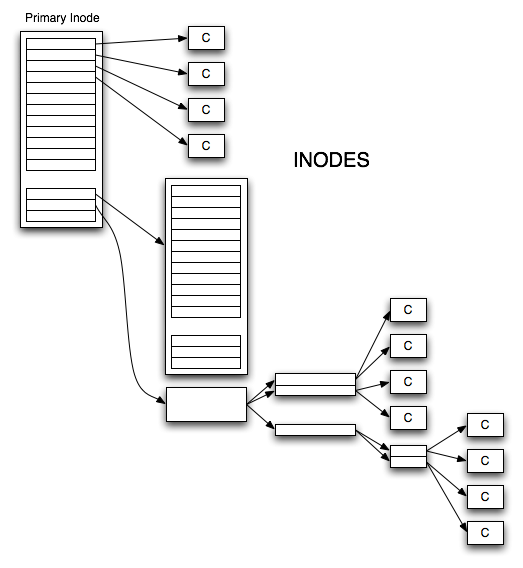
\includegraphics[width=0.6\textwidth]{inodes.png}
\end{figure} 

Cada inodo en el sistema de archivos Minix 1 se identifica por un n\'umero entero positivo entre 1 y 65536. Esto permite por
ejemplo que la organizaci\'on de los directorios siga un esquema de \'arbol (aunque existe la noci\'on de \textit{hard} y \textit{soft}
links en Minix 1, por simplicidad no fueron implementados): Cada inodo de directorio almacena en sus zonas de datos entradas de 32 bytes
que consisten en:

\begin{itemize}
	\item 2 bytes para el numero de inodo correspondiente al hijo.
	\item 30 nombres para el pedazo del nombre del hijo.
\end{itemize}

Por ejemplo, si tuvieramos el archivo \url{/docs/docs/archivo.txt}, \texttt{archivo.txt} ser\'ia el nombre con el que identificar\'iamos en
el inodo del segundo \texttt{docs} al inodo del archivo final. La organizaci\'on es entonces jer\'arquica separada por caracteres de barra
como es usual en los sistemas UNIX.

Por \'ultimo es necesario considerar los archivos correspondientes a drivers. Los drivers en Minix se identifican con dos n\'umeros, el
n\'umero major (que indica el tipo de dispositivo) y el n\'umero minor (que indica una instancia del tipo de dispositivo dado por el otro
n\'umero). Estos dos valores se almacenan en las dos primeras zonas del inodo en disco.

La distinci\'on entre los distintos tipos de inodo es posible gracias a un flag de identificaci\'on que es parte del inodo. Adem\'as de esto
el inodo en disco mantiene el tama\~no en bytes del archivo.

Finalmente, es necesario mantener ciertos datos sobre la partici\'on utilizada: por ejemplo que inodos est\'an usados o no, la informaci\'on
de cada inodo en una secci\'on encontrable a priori de iniciar la partici\'on, y que zonas en disco est\'an o no libres.

Para esto, toda partici\'on Minix 1 de disco inicia con el bootblock (que contiene la informaci\'on para bootear el sistema operativo en disco
duro, que en nuestro caso no utilizamos puesto que se bootea directamente mediante el diskette) al cual le sigue el denominado \textit{super block}. El super bloque inicia entonces en la segunda zona (Sector n\'umero 3) y contiene la siguiente informaci\'on:

\begin{itemize}
	\item La cantidad de inodos en la partici\'on actual.
	\item La cantidad de zonas de datos disponibles en la partici\'on actual.
	\item Cantidad de bloques correspondientes al mapa de bits de inodos.
	\item Cantidad de bloques correspondientes al mapa de bits de zonas de datos libres.
	\item Zona de inicio de las zonas de datos.
	\item Valor $c$ tal que $2^c$ corresponde al tama\~no en zonas del espacio de datos del disco.
	\item Tama\~no m\'aximo de archivo.
	\item Valor m\'agico que identifica esta partici\'on. En el caso de MINIX 1 este valor es $0x138F$
\end{itemize}

Posteriormente a este super bloque, viene un mapa de bits que codifica que inodos est\'an o no libres, y luego un mapa de bits que codifica
que zonas de datos est\'an o no libres. Ambos mapas de bits son cargados a memoria cuando se inicializa el super bloque en memoria con el
pr\'oposito de utilizar la estructura \texttt{bitset} descripta en la secci\'on~\ref{sec::memory} para administrar estos espacios. Finalmente,
lo que sigue es la zona de inodos: un arreglo contiguo de zonas que almacenan la metainformaci\'on de cada inodo del sistema, o espacio libre
si ese inodo no esta asignado. Puesto que la estructura en disco de un inodo consiste de 32 bytes, la cantidad de estas que entra en 1024 bytes
es entera y nunca cruza un borde de zona. Finalmente, a esto sigue las zonas de datos.

Un esquema de esta organizaci\'on de las primeras zonas del disco se puede ver en la Figura~\ref{fig::superblock}.

\begin{figure}[H]
	\caption{Organizaci\'on de las primeras zonas de una partici\'on de Minix.}
	\label{fig::superblock}
	\centering
	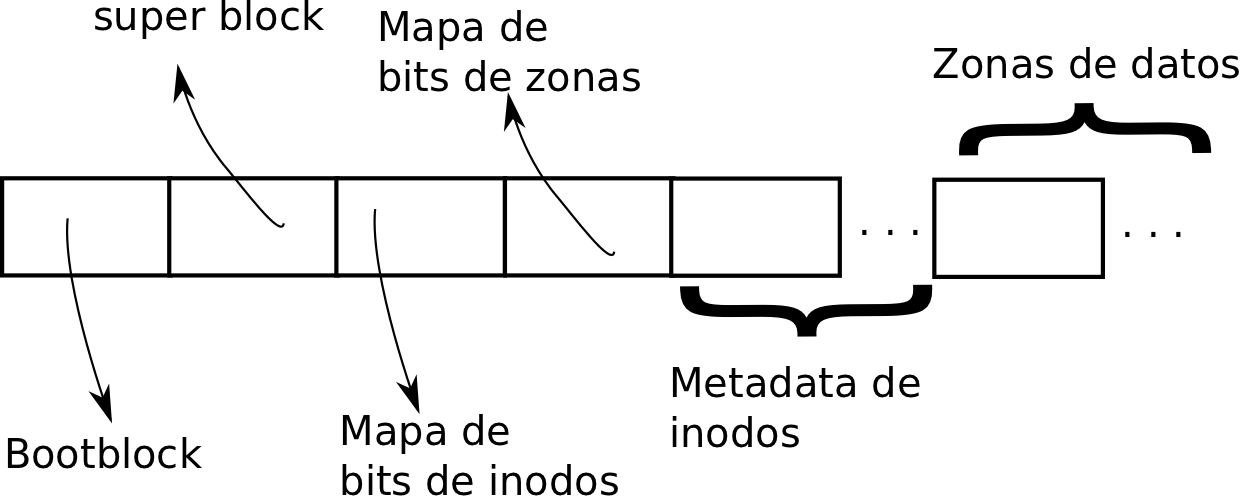
\includegraphics[width=0.6\textwidth]{superblock.png}
\end{figure} 

Otro motivo para utilizar este sistema de archivos es que en el entorno de desarrollo utilizado se disponen de herramientas para crear archivos
que contengan una partici\'on de Minix 1: En particular estamos hablando del comando \texttt{mkfs.minix}. De esta manera, podemos utilizar 
este comando y comandos espec\'ificos para armar im\'agenes de disco para el simulador Bochs para crear una im\'agen de disco con el sistema
de archivos valido y que contenga los valores que deseemos. Esto en particular nos fue muy \'util para resolver problemas no documentados sobre
el sistema de archivos y para adem\'as poder testear el c\'odigo de sistema de archivos por separado al c\'odigo del resto del Sistema Operativo
(mejorando as\'i la modularidad).

Por \'ultimo ahondaremos en dos detalles implementativos: La noci\'on de Virtual Filesystem y la noci\'on de cache de buffers y cache de
inodos.

\subsection{Virtual Filesystem}

La idea de un sistema de archivos virtual es proveer una abstracci\'on por sobre la implementaci\'on particular del sistema de archivos de
manera de poder trabajar de manera general sobre ellos. En nuestro caso, la capa de abstracci\'on se provee mediante las nociones de inodo,
superbloque y file object. Las dos primeras nociones son id\'enticas a las de Minix, con modificaciones que veremos posteriormente. La noci\'on
de file object es la de una instancia de un inodo abierto. Esto sirve por ejemplo para mantener la idea de que estamos leyendo un cierto offset dentro de un inodo y que esto es independiente del inodo en si (que representa un archivo).

La modificaci\'on m\'as importante es que cada uno de estos tres valores provee una abstracci\'on en la forma de una serie de funciones:

\begin{itemize}
	\item El super bloque debe ser capaz de crear, leer de disco, escribir a disco y mantener la consistencia de los inodos en una partici\'on,
	sea esta la que sea. En el caso de Minix por ejemplo se ocupa de mantener la consistencia de los mapas de bits con los inodos en uso y las
	zonas de datos disponibles, y de mantener los metadatos de cada inodo coherentes con su representaci\'on en los caches de memoria RAM.
	\item El inodo debe ser capaz de operar sobre la noci\'on de archivo. Por ejemplo, un inodo de directorio debe proveer funciones para
	buscar el inodo de un subarchivo directo en la jerarqu\'ia, crear subdirectorios y subarchivos, borrar subarchivos, etc. Debe proveer
	adem\'as una abstracci\'on con respecto a que operaciones de acci\'on se pueden realizar sobre \'el: que quiere decir leerlo, escribirlo,
	etc.
	\item Un file object no provee m\'as abstracci\'on que la de ser una instancia de un inodo abierto. Mantiene \'indices dentro del mismo y
	conoce las operaciones que se pueden realizar. Su prop\'osito por sobre todo es ser el objeto interfaz entre los procesos (mediante las
	llamadas a sistema) y el sistema de archivos en si.
\end{itemize}

De esta manera, se tiene una abstracci\'on general que permite por ejemplo el manejo gen\'erico de archivos con un mismo conjunto de llamadas
a sistema (que describiremos en ~\ref{sec::filesystem_syscalls}.

\subsection{Caches de disco y de inodos}

Para evitar problemas de fragmentaci\'on de la memoria, se mantiene un cache de inodos. Esto quiere decir que cuando el sistema operativo
necesita un inodo, busca si uno ya preasignado fue liberado. Si fue liberado, lo utiliza, sino, crea uno nuevo y lo agrega a una lista. Esta
lista es responsabilidad del superbloque de la partici\'on, que la mantiene. De esta manera, no se fragmenta la memoria producto de crear y
liberar muchas veces un inodo, y se mejora la performance y se mantiene una interfaz m\'as simple. Cada inodo lleva para este prop\'osito un
contador de instancias en uso. Si bien el sistema de archivos es \textit{single-threaded} como esta implementado (es decir, se producir\'ian
condiciones de carrera si dos instancias de un proceso por ejemplo actuaran sobre el mismo archivo), este contador de instancias de uso se
podr\'ia utilizar posteriormente para mantener una sola instancia sincronizada en memoria del inodo, manteniendose entonces la consistencia
del sistema de archivos (usandose para ello por ejemplo un esquema de sincronizaci\'on por sem\'aforos).

Para abstraer los accesos a disco, que se hacen por sectores, se implement\'o adem\'as un cache de buffers, muy similar al disponible por
ejemplo en Unix System V (ver~\cite{systemv}). Este cache consiste en una serie de buffers de tama\~no de una zona, linkeados entre si con
una lista enlazada. Cada buffer sabe a que zona y con que desplazamiento esta actuando, y adem\'as sabe si los datos est\'an o no sincronizados
con el disco duro (ya que sabe que operaci\'on se esta realizando sobre \'el). Cuando se desea escribir a disco solamente es necesario indicar
el bloque y offset deseados, y pasar los datos. El cache de buffers se ocupa de buscar el buffer correspondiente si ya esta abierto, y si no
es as\'i se ocupa de encontrar un buffer libre y desalojarlo como corresponda (por ejemplo escribiendolo a disco si estaba sucio). En \'ultima
instancia si no encuentra ninguno lo que hace es agregar un nuevo buffer a la lista enlazada de buffers libres.

Adicionalmente, se mantiene una lista de buffers sucios y a que inodo corresponde cada uno, de manera de poder, en caso de ser pertinente, bajar
los datos a disco de los buffers sucios correspondientes a un inodo (por ejemplo, cuando se realiza un \texttt{close} o un \texttt{flush}).

\subsection{Llamadas de sistema operativo}
\label{sec::filesystem_syscalls}
